% Options for packages loaded elsewhere
\PassOptionsToPackage{unicode}{hyperref}
\PassOptionsToPackage{hyphens}{url}
\PassOptionsToPackage{dvipsnames,svgnames,x11names}{xcolor}
%
\documentclass[
  10pt,
  letterpaper]{article}

\usepackage{amsmath,amssymb}
\usepackage{lmodern}
\usepackage{iftex}
\ifPDFTeX
  \usepackage[T1]{fontenc}
  \usepackage[utf8]{inputenc}
  \usepackage{textcomp} % provide euro and other symbols
\else % if luatex or xetex
  \usepackage{unicode-math}
  \defaultfontfeatures{Scale=MatchLowercase}
  \defaultfontfeatures[\rmfamily]{Ligatures=TeX,Scale=1}
  \setmainfont[]{Charis SIL}
  \setmathfont[]{Monaco}
\fi
% Use upquote if available, for straight quotes in verbatim environments
\IfFileExists{upquote.sty}{\usepackage{upquote}}{}
\IfFileExists{microtype.sty}{% use microtype if available
  \usepackage[]{microtype}
  \UseMicrotypeSet[protrusion]{basicmath} % disable protrusion for tt fonts
}{}
\makeatletter
\@ifundefined{KOMAClassName}{% if non-KOMA class
  \IfFileExists{parskip.sty}{%
    \usepackage{parskip}
  }{% else
    \setlength{\parindent}{0pt}
    \setlength{\parskip}{6pt plus 2pt minus 1pt}}
}{% if KOMA class
  \KOMAoptions{parskip=half}}
\makeatother
\usepackage{xcolor}
\usepackage[margin = 1in]{geometry}
\setlength{\emergencystretch}{3em} % prevent overfull lines
\setcounter{secnumdepth}{-\maxdimen} % remove section numbering
% Make \paragraph and \subparagraph free-standing
\ifx\paragraph\undefined\else
  \let\oldparagraph\paragraph
  \renewcommand{\paragraph}[1]{\oldparagraph{#1}\mbox{}}
\fi
\ifx\subparagraph\undefined\else
  \let\oldsubparagraph\subparagraph
  \renewcommand{\subparagraph}[1]{\oldsubparagraph{#1}\mbox{}}
\fi

\usepackage{color}
\usepackage{fancyvrb}
\newcommand{\VerbBar}{|}
\newcommand{\VERB}{\Verb[commandchars=\\\{\}]}
\DefineVerbatimEnvironment{Highlighting}{Verbatim}{commandchars=\\\{\}}
% Add ',fontsize=\small' for more characters per line
\usepackage{framed}
\definecolor{shadecolor}{RGB}{241,243,245}
\newenvironment{Shaded}{\begin{snugshade}}{\end{snugshade}}
\newcommand{\AlertTok}[1]{\textcolor[rgb]{0.68,0.00,0.00}{#1}}
\newcommand{\AnnotationTok}[1]{\textcolor[rgb]{0.37,0.37,0.37}{#1}}
\newcommand{\AttributeTok}[1]{\textcolor[rgb]{0.40,0.45,0.13}{#1}}
\newcommand{\BaseNTok}[1]{\textcolor[rgb]{0.68,0.00,0.00}{#1}}
\newcommand{\BuiltInTok}[1]{\textcolor[rgb]{0.00,0.23,0.31}{#1}}
\newcommand{\CharTok}[1]{\textcolor[rgb]{0.13,0.47,0.30}{#1}}
\newcommand{\CommentTok}[1]{\textcolor[rgb]{0.37,0.37,0.37}{#1}}
\newcommand{\CommentVarTok}[1]{\textcolor[rgb]{0.37,0.37,0.37}{\textit{#1}}}
\newcommand{\ConstantTok}[1]{\textcolor[rgb]{0.56,0.35,0.01}{#1}}
\newcommand{\ControlFlowTok}[1]{\textcolor[rgb]{0.00,0.23,0.31}{#1}}
\newcommand{\DataTypeTok}[1]{\textcolor[rgb]{0.68,0.00,0.00}{#1}}
\newcommand{\DecValTok}[1]{\textcolor[rgb]{0.68,0.00,0.00}{#1}}
\newcommand{\DocumentationTok}[1]{\textcolor[rgb]{0.37,0.37,0.37}{\textit{#1}}}
\newcommand{\ErrorTok}[1]{\textcolor[rgb]{0.68,0.00,0.00}{#1}}
\newcommand{\ExtensionTok}[1]{\textcolor[rgb]{0.00,0.23,0.31}{#1}}
\newcommand{\FloatTok}[1]{\textcolor[rgb]{0.68,0.00,0.00}{#1}}
\newcommand{\FunctionTok}[1]{\textcolor[rgb]{0.28,0.35,0.67}{#1}}
\newcommand{\ImportTok}[1]{\textcolor[rgb]{0.00,0.46,0.62}{#1}}
\newcommand{\InformationTok}[1]{\textcolor[rgb]{0.37,0.37,0.37}{#1}}
\newcommand{\KeywordTok}[1]{\textcolor[rgb]{0.00,0.23,0.31}{#1}}
\newcommand{\NormalTok}[1]{\textcolor[rgb]{0.00,0.23,0.31}{#1}}
\newcommand{\OperatorTok}[1]{\textcolor[rgb]{0.37,0.37,0.37}{#1}}
\newcommand{\OtherTok}[1]{\textcolor[rgb]{0.00,0.23,0.31}{#1}}
\newcommand{\PreprocessorTok}[1]{\textcolor[rgb]{0.68,0.00,0.00}{#1}}
\newcommand{\RegionMarkerTok}[1]{\textcolor[rgb]{0.00,0.23,0.31}{#1}}
\newcommand{\SpecialCharTok}[1]{\textcolor[rgb]{0.37,0.37,0.37}{#1}}
\newcommand{\SpecialStringTok}[1]{\textcolor[rgb]{0.13,0.47,0.30}{#1}}
\newcommand{\StringTok}[1]{\textcolor[rgb]{0.13,0.47,0.30}{#1}}
\newcommand{\VariableTok}[1]{\textcolor[rgb]{0.07,0.07,0.07}{#1}}
\newcommand{\VerbatimStringTok}[1]{\textcolor[rgb]{0.13,0.47,0.30}{#1}}
\newcommand{\WarningTok}[1]{\textcolor[rgb]{0.37,0.37,0.37}{\textit{#1}}}

\providecommand{\tightlist}{%
  \setlength{\itemsep}{0pt}\setlength{\parskip}{0pt}}\usepackage{longtable,booktabs,array}
\usepackage{calc} % for calculating minipage widths
% Correct order of tables after \paragraph or \subparagraph
\usepackage{etoolbox}
\makeatletter
\patchcmd\longtable{\par}{\if@noskipsec\mbox{}\fi\par}{}{}
\makeatother
% Allow footnotes in longtable head/foot
\IfFileExists{footnotehyper.sty}{\usepackage{footnotehyper}}{\usepackage{footnote}}
\makesavenoteenv{longtable}
\usepackage{graphicx}
\makeatletter
\def\maxwidth{\ifdim\Gin@nat@width>\linewidth\linewidth\else\Gin@nat@width\fi}
\def\maxheight{\ifdim\Gin@nat@height>\textheight\textheight\else\Gin@nat@height\fi}
\makeatother
% Scale images if necessary, so that they will not overflow the page
% margins by default, and it is still possible to overwrite the defaults
% using explicit options in \includegraphics[width, height, ...]{}
\setkeys{Gin}{width=\maxwidth,height=\maxheight,keepaspectratio}
% Set default figure placement to htbp
\makeatletter
\def\fps@figure{htbp}
\makeatother

\usepackage{tabularx}
\usepackage{threeparttable}
\usepackage{booktabs}
\usepackage{tipa}
\let\Oldtexttt\texttt
\renewcommand\texttt[1]{{\ttfamily\color{BrickRed}#1}}
\usepackage{authoraftertitle}
\usepackage{fancyhdr}
\pagestyle{fancy}
\rfoot{\copyright Matt Hunt Gardner}
\cfoot{\thepage}
\lhead{Doing LVC with \textit{R}: \MyTitle}
\rhead{}
\makeatletter
\@ifpackageloaded{tcolorbox}{}{\usepackage[many]{tcolorbox}}
\@ifpackageloaded{fontawesome5}{}{\usepackage{fontawesome5}}
\definecolor{quarto-callout-color}{HTML}{909090}
\definecolor{quarto-callout-note-color}{HTML}{0758E5}
\definecolor{quarto-callout-important-color}{HTML}{CC1914}
\definecolor{quarto-callout-warning-color}{HTML}{EB9113}
\definecolor{quarto-callout-tip-color}{HTML}{00A047}
\definecolor{quarto-callout-caution-color}{HTML}{FC5300}
\definecolor{quarto-callout-color-frame}{HTML}{acacac}
\definecolor{quarto-callout-note-color-frame}{HTML}{4582ec}
\definecolor{quarto-callout-important-color-frame}{HTML}{d9534f}
\definecolor{quarto-callout-warning-color-frame}{HTML}{f0ad4e}
\definecolor{quarto-callout-tip-color-frame}{HTML}{02b875}
\definecolor{quarto-callout-caution-color-frame}{HTML}{fd7e14}
\makeatother
\makeatletter
\makeatother
\makeatletter
\makeatother
\makeatletter
\@ifpackageloaded{caption}{}{\usepackage{caption}}
\AtBeginDocument{%
\ifdefined\contentsname
  \renewcommand*\contentsname{Table of contents}
\else
  \newcommand\contentsname{Table of contents}
\fi
\ifdefined\listfigurename
  \renewcommand*\listfigurename{List of Figures}
\else
  \newcommand\listfigurename{List of Figures}
\fi
\ifdefined\listtablename
  \renewcommand*\listtablename{List of Tables}
\else
  \newcommand\listtablename{List of Tables}
\fi
\ifdefined\figurename
  \renewcommand*\figurename{Figure}
\else
  \newcommand\figurename{Figure}
\fi
\ifdefined\tablename
  \renewcommand*\tablename{Table}
\else
  \newcommand\tablename{Table}
\fi
}
\@ifpackageloaded{float}{}{\usepackage{float}}
\floatstyle{ruled}
\@ifundefined{c@chapter}{\newfloat{codelisting}{h}{lop}}{\newfloat{codelisting}{h}{lop}[chapter]}
\floatname{codelisting}{Listing}
\newcommand*\listoflistings{\listof{codelisting}{List of Listings}}
\makeatother
\makeatletter
\@ifpackageloaded{caption}{}{\usepackage{caption}}
\@ifpackageloaded{subcaption}{}{\usepackage{subcaption}}
\makeatother
\makeatletter
\@ifpackageloaded{tcolorbox}{}{\usepackage[many]{tcolorbox}}
\makeatother
\makeatletter
\@ifundefined{shadecolor}{\definecolor{shadecolor}{rgb}{.97, .97, .97}}
\makeatother
\makeatletter
\makeatother
\ifLuaTeX
  \usepackage{selnolig}  % disable illegal ligatures
\fi
\IfFileExists{bookmark.sty}{\usepackage{bookmark}}{\usepackage{hyperref}}
\IfFileExists{xurl.sty}{\usepackage{xurl}}{} % add URL line breaks if available
\urlstyle{same} % disable monospaced font for URLs
% Make links footnotes instead of hotlinks:
\DeclareRobustCommand{\href}[2]{#2\footnote{\url{#1}}}
\hypersetup{
  pdftitle={Proportions for ggplot2},
  pdfauthor={Matt Hunt Gardner},
  colorlinks=true,
  linkcolor={blue},
  filecolor={Maroon},
  citecolor={Blue},
  urlcolor={Blue},
  pdfcreator={LaTeX via pandoc}}

\title{Proportions for \texttt{ggplot2}}
\usepackage{etoolbox}
\makeatletter
\providecommand{\subtitle}[1]{% add subtitle to \maketitle
  \apptocmd{\@title}{\par {\large #1 \par}}{}{}
}
\makeatother
\subtitle{from
\href{https://lingmethodshub.github.io/content/R/lvc_r/}{Doing LVC with
\emph{R}}}
\author{Matt Hunt Gardner}
\date{2/16/23}

\begin{document}
\maketitle
\ifdefined\Shaded\renewenvironment{Shaded}{\begin{tcolorbox}[borderline west={3pt}{0pt}{shadecolor}, enhanced, boxrule=0pt, breakable, sharp corners, frame hidden, interior hidden]}{\end{tcolorbox}}\fi

There are two main ways to make graphs in \emph{R}. The first is using
the standard graphing capabilities of \emph{R}. The second is using a
much more sophisticated and customizable graphics package called
\texttt{ggplot2}. Describing the ins and outs of the \texttt{ggplot2}
package is beyond the scope of these instructions, but what these
instructions can do is teach you how to organize your summary statistics
in such a way that they are usable by \texttt{ggplot2}.

Why is there a separate section on preparing summary statistics for
\texttt{ggplot2}? It is \texttt{ggplot2} expects summary statistics to
be organized in a way that is non-intuitive to us as sociolinguists.
When we represent summary statistics we usually represent them like
cross-tabs, for example:

\hypertarget{tbl-normal}{}
\begin{longtable}[]{@{}
  >{\raggedright\arraybackslash}p{(\columnwidth - 12\tabcolsep) * \real{0.1429}}
  >{\raggedright\arraybackslash}p{(\columnwidth - 12\tabcolsep) * \real{0.1429}}
  >{\raggedright\arraybackslash}p{(\columnwidth - 12\tabcolsep) * \real{0.1429}}
  >{\raggedright\arraybackslash}p{(\columnwidth - 12\tabcolsep) * \real{0.1429}}
  >{\raggedright\arraybackslash}p{(\columnwidth - 12\tabcolsep) * \real{0.1429}}
  >{\raggedright\arraybackslash}p{(\columnwidth - 12\tabcolsep) * \real{0.1429}}
  >{\raggedright\arraybackslash}p{(\columnwidth - 12\tabcolsep) * \real{0.1429}}@{}}
\caption{\label{tbl-normal}Percentage of deleted (t, d) tokens by Age
Group and Sex in Cape Breton English}\tabularnewline
\toprule()
\begin{minipage}[b]{\linewidth}\raggedright
\end{minipage} & \begin{minipage}[b]{\linewidth}\raggedright
\textbf{Female}
\end{minipage} & \begin{minipage}[b]{\linewidth}\raggedright
\end{minipage} & \begin{minipage}[b]{\linewidth}\raggedright
\textbf{Male}
\end{minipage} & \begin{minipage}[b]{\linewidth}\raggedright
\end{minipage} & \begin{minipage}[b]{\linewidth}\raggedright
\textbf{Total}
\end{minipage} & \begin{minipage}[b]{\linewidth}\raggedright
\end{minipage} \\
\midrule()
\endfirsthead
\toprule()
\begin{minipage}[b]{\linewidth}\raggedright
\end{minipage} & \begin{minipage}[b]{\linewidth}\raggedright
\textbf{Female}
\end{minipage} & \begin{minipage}[b]{\linewidth}\raggedright
\end{minipage} & \begin{minipage}[b]{\linewidth}\raggedright
\textbf{Male}
\end{minipage} & \begin{minipage}[b]{\linewidth}\raggedright
\end{minipage} & \begin{minipage}[b]{\linewidth}\raggedright
\textbf{Total}
\end{minipage} & \begin{minipage}[b]{\linewidth}\raggedright
\end{minipage} \\
\midrule()
\endhead
Age Group & n & \% Deletion & n & \% Deletion & n & \% Deletion \\
Young & 271 & 27 & 357 & 34 & 628 & \textbf{31} \\
Middle & 238 & 31 & 122 & 43 & 360 & \textbf{35} \\
Old & 150 & 29 & 51 & 47 & 201 & \textbf{33} \\
\textbf{Total} & \textbf{659} & \textbf{28} & \textbf{530} & \textbf{37}
& \textbf{1,189} & \textbf{32} \\
\bottomrule()
\end{longtable}

In the above table there are variables both as rows (here
\texttt{Age.Group}) and columns (here \texttt{Sex}). If I was going to
create a chart in \emph{Excel} of summary statistics this is how I would
naturally make it. This is how data is presented in manuscripts, it is
also how it is presented in \emph{Goldvarb}, and it is how it is
presented to us by the \texttt{prop.table()} function. It is NOT how
\texttt{ggplot2} wants your data to be organized. For \texttt{ggplot2}
each variable has to exist in its own individual column --- much closer
to the organization of the \texttt{ftable()} or what is produced using
\texttt{tidy} methods.

In order to create this kind of organization (if not using \texttt{tidy}
methods) you need to ``melt'' the \texttt{prop.table()} using the
function \texttt{melt()} in the package \texttt{reshape2}. You'll do
this in two steps. First you create a new object \texttt{td.prop}, which
is the proportion table of the levels of \texttt{Dep.Var} for each level
of \texttt{Age.Group} and \texttt{Sex}, just like the table above. Then
you ``melt'' that table using the function \texttt{melt()}, and assign
this new table to a new object \texttt{td.prop.melt}.

\begin{tcolorbox}[enhanced jigsaw, rightrule=.15mm, colback=white, opacityback=0, toprule=.15mm, leftrule=.75mm, arc=.35mm, breakable, bottomtitle=1mm, colframe=quarto-callout-tip-color-frame, left=2mm, colbacktitle=quarto-callout-tip-color!10!white, opacitybacktitle=0.6, toptitle=1mm, titlerule=0mm, coltitle=black, title=\textcolor{quarto-callout-tip-color}{\faLightbulb}\hspace{0.5em}{Get the data first}, bottomrule=.15mm]

If you don't have the \texttt{td} data loaded in \emph{R}, go back to
\href{https://lingmethodshub.github.io/content/R/lvc_r/050_lvcr.html}{Doing
it all again, but \texttt{tidy}} and run the code.

\end{tcolorbox}

\begin{Shaded}
\begin{Highlighting}[]
\CommentTok{\# Create object td.prop as proportion table of}
\CommentTok{\# each level of Dep.Var for each level of}
\CommentTok{\# Age.Group and Sex}
\NormalTok{td.prop }\OtherTok{\textless{}{-}} \FunctionTok{prop.table}\NormalTok{(}\FunctionTok{table}\NormalTok{(td}\SpecialCharTok{$}\NormalTok{Age.Group, td}\SpecialCharTok{$}\NormalTok{Sex, td}\SpecialCharTok{$}\NormalTok{Dep.Var),}
    \AttributeTok{margin =} \FunctionTok{c}\NormalTok{(}\DecValTok{1}\NormalTok{, }\DecValTok{2}\NormalTok{))}

\CommentTok{\# Melt td.prop}
\FunctionTok{library}\NormalTok{(reshape2)}
\NormalTok{td.prop.melt }\OtherTok{\textless{}{-}} \FunctionTok{melt}\NormalTok{(td.prop)}

\CommentTok{\# View first six lines of td.prop.melt}
\FunctionTok{head}\NormalTok{(td.prop.melt)}
\end{Highlighting}
\end{Shaded}

\begin{verbatim}
    Var1 Var2     Var3     value
1    Old    F Deletion 0.2866667
2 Middle    F Deletion 0.3067227
3  Young    F Deletion 0.2656827
4    Old    M Deletion 0.4705882
5 Middle    M Deletion 0.4262295
6  Young    M Deletion 0.3417367
\end{verbatim}

This new melted table does not contain informative column names, so you
add those as the third step.

\begin{Shaded}
\begin{Highlighting}[]
\CommentTok{\# Create column names for td.prop.melt}
\FunctionTok{colnames}\NormalTok{(td.prop.melt) }\OtherTok{\textless{}{-}} \FunctionTok{c}\NormalTok{(}\StringTok{"Age.Group"}\NormalTok{, }\StringTok{"Sex"}\NormalTok{, }\StringTok{"Dep.Var"}\NormalTok{,}
    \StringTok{"Percent"}\NormalTok{)}
\CommentTok{\# View first six lines of td.prop.melt}
\FunctionTok{head}\NormalTok{(td.prop.melt)}
\end{Highlighting}
\end{Shaded}

\begin{verbatim}
  Age.Group Sex  Dep.Var   Percent
1       Old   F Deletion 0.2866667
2    Middle   F Deletion 0.3067227
3     Young   F Deletion 0.2656827
4       Old   M Deletion 0.4705882
5    Middle   M Deletion 0.4262295
6     Young   M Deletion 0.3417367
\end{verbatim}

An alternative way to melt the columns is to save the proportion table
as a new tab-delimited-text file. You might want to do this anyway, as
having a separate file containing summary statistics may be useful to
you. One use I have for tab-delimited-text file versions of my summary
statistics is that they are much easier for copying and pasting. If you
copy and paste from the \emph{R} console window there is an inconsistent
number of space characters between columns (e.g., above there are five
space characters between \texttt{1} and \texttt{Young}, four between
\texttt{2} and \texttt{Middle}, and five between \texttt{3}
and\texttt{Old}). If you save that same table to a text file you can
specify that you want each cell separated by a tab character instead.

\begin{Shaded}
\begin{Highlighting}[]
\CommentTok{\# Create object td.prop as proportion table of}
\CommentTok{\# each level of Dep.Var for each level of}
\CommentTok{\# Age.Group and Sex}
\NormalTok{td.prop }\OtherTok{\textless{}{-}} \FunctionTok{prop.table}\NormalTok{(}\FunctionTok{table}\NormalTok{(td}\SpecialCharTok{$}\NormalTok{Age.Group, td}\SpecialCharTok{$}\NormalTok{Sex, td}\SpecialCharTok{$}\NormalTok{Dep.Var),}
    \AttributeTok{margin =} \FunctionTok{c}\NormalTok{(}\DecValTok{1}\NormalTok{, }\DecValTok{2}\NormalTok{))}

\CommentTok{\# Melt td.prop}
\FunctionTok{library}\NormalTok{(reshape2)}
\NormalTok{td.prop.melt }\OtherTok{\textless{}{-}} \FunctionTok{melt}\NormalTok{(td.prop)}

\CommentTok{\# Create column names for td.prop.melt}
\FunctionTok{colnames}\NormalTok{(td.prop.melt) }\OtherTok{\textless{}{-}} \FunctionTok{c}\NormalTok{(}\StringTok{"Age.Group"}\NormalTok{, }\StringTok{"Sex"}\NormalTok{, }\StringTok{"Dep.Var"}\NormalTok{,}
    \StringTok{"Percent"}\NormalTok{)}

\CommentTok{\# Write td.prop.melt to file}
\FunctionTok{write.table}\NormalTok{(td.prop.melt, }\AttributeTok{file =} \StringTok{"Data/summaryAgeGroupSexMelted.txt"}\NormalTok{,}
    \AttributeTok{quote =} \ConstantTok{FALSE}\NormalTok{, }\AttributeTok{sep =} \StringTok{"}\SpecialCharTok{\textbackslash{}t}\StringTok{"}\NormalTok{, }\AttributeTok{row.names =} \ConstantTok{FALSE}\NormalTok{)}


\CommentTok{\# Write td.prop to file (with automatic melting)}
\FunctionTok{write.table}\NormalTok{(td.prop, }\AttributeTok{file =} \StringTok{"Data/summaryAgeGroupSex.txt"}\NormalTok{,}
    \AttributeTok{quote =} \ConstantTok{FALSE}\NormalTok{, }\AttributeTok{sep =} \StringTok{"}\SpecialCharTok{\textbackslash{}t}\StringTok{"}\NormalTok{, }\AttributeTok{row.names =} \ConstantTok{FALSE}\NormalTok{)}
\end{Highlighting}
\end{Shaded}

The two \texttt{write.table()} functions above produce the exact same
tab-delimited-text file. The one difference between them is that the
melted table (e.g., \texttt{summaryAgeGroupSexMelted.txt}) includes
column names.

\begin{figure}

{\centering 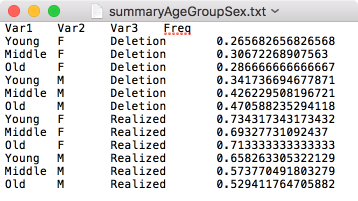
\includegraphics{images/summaryAgeGroupSex.png}

}

\caption{\label{fig-notmelted}Not Melted}

\end{figure}

\begin{figure}

{\centering 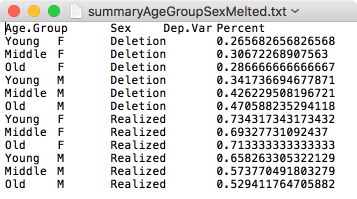
\includegraphics{images/summaryAgeGroupSexMelted.png}

}

\caption{\label{fig-melted}Melted}

\end{figure}

When the \texttt{write.table()} melts the proportion table for you it
does not create the new column names. For this reason, I like to melt
proportion tables before I save them so that I have the opportunity to
name the table's columns. In the \texttt{write.table()} functions above
you first specify the object you want to write to a text file, then you
specify what you want to call that file and where you want it to be
created. Here I've named the files \texttt{summaryAgeGroupSexMelted.txt}
and \texttt{summaryAgeGroupSex.txt} and saved it in a subfolder called
\texttt{Data} in the same folder in which my \emph{R} script is saved.
You can save your file anywhere on your computer and call it whatever
you want. You can specify any file path here. For example, I could have
written \texttt{\textasciitilde{}/Documents/My\ Project/Data} to
indicate a folder called \texttt{Data} in a folder called
\texttt{My\ Project} in my \texttt{Documents} folder on root drive of my
Mac computer. If you are running a PC your folder structure will likely
start with \texttt{"C:/\textbackslash{}dots"}. In the function you
specify that \texttt{quote\ =\ FALSE}. If you specify \texttt{TRUE},
\emph{R} will put quotation marks around the values in each cell. I have
never needed this. You further specify that the separator between cells
in the same row is a tab, \texttt{sep="\textbackslash{}t"}, which
creates a tab-delimited-text file (.txt). If you wanted to create a
comma-separated-value table (.csv) you would instead specify
\texttt{sep=","} and change the file extension from \texttt{".txt"} to
\texttt{".csv"}. Finally, you specify that \texttt{row.names\ =\ FALSE}
because there are no row names in this table, just column names.

If you've saved a summary statistics file previously and want to read it
into \emph{R} for use with \texttt{ggplot2}, you can use the same
procedure as you used for reading in your data file.

\begin{Shaded}
\begin{Highlighting}[]
\CommentTok{\# Read in Summary Statistics File}
\NormalTok{td.AgeSex }\OtherTok{\textless{}{-}} \FunctionTok{read.delim}\NormalTok{(}\StringTok{"Data/summaryAgeGroupSexMelted.txt"}\NormalTok{)}
\end{Highlighting}
\end{Shaded}

Here's an example of a basic \texttt{ggplot2} line graph that can be
made with the above summary statistics. The first three steps are only
necessary if you didn't read in the summary statistics file above.

\begin{Shaded}
\begin{Highlighting}[]
\CommentTok{\# Create object td.prop as proportion table of each level of Dep.Var }
\CommentTok{\# for each level of Age.Group and Sex}
\NormalTok{td.prop }\OtherTok{\textless{}{-}}\FunctionTok{prop.table}\NormalTok{(}\FunctionTok{table}\NormalTok{(td}\SpecialCharTok{$}\NormalTok{Age.Group, td}\SpecialCharTok{$}\NormalTok{Sex, td}\SpecialCharTok{$}\NormalTok{Dep.Var), }\AttributeTok{margin=}\FunctionTok{c}\NormalTok{(}\DecValTok{1}\NormalTok{,}\DecValTok{2}\NormalTok{))}

\CommentTok{\# Melt td.prop  }
\FunctionTok{library}\NormalTok{(reshape2)}
\NormalTok{td.AgeSex }\OtherTok{\textless{}{-}}\FunctionTok{melt}\NormalTok{(td.prop)}

\CommentTok{\# Create column names for td.prop.melt}
\FunctionTok{colnames}\NormalTok{(td.AgeSex) }\OtherTok{\textless{}{-}}\FunctionTok{c}\NormalTok{(}\StringTok{"Age.Group"}\NormalTok{, }\StringTok{"Sex"}\NormalTok{, }\StringTok{"Dep.Var"}\NormalTok{, }\StringTok{"Percent"}\NormalTok{)}

\CommentTok{\# Reorder Age.Group}
\NormalTok{td.AgeSex}\SpecialCharTok{$}\NormalTok{Age.Group }\OtherTok{\textless{}{-}}\FunctionTok{factor}\NormalTok{(td.AgeSex}\SpecialCharTok{$}\NormalTok{Age.Group, }\AttributeTok{levels =} \FunctionTok{c}\NormalTok{(}\StringTok{"Old"}\NormalTok{, }\StringTok{"Middle"}\NormalTok{, }\StringTok{"Young"}\NormalTok{))}

\CommentTok{\# Create basic ggplot2 line graph of the proportion of deletion by Age.Group, }
\CommentTok{\# with lines separated by Sex}
\FunctionTok{library}\NormalTok{(ggplot2)}
\FunctionTok{qplot}\NormalTok{(}\AttributeTok{data =}\NormalTok{ td.AgeSex[td.AgeSex}\SpecialCharTok{$}\NormalTok{Dep.Var }\SpecialCharTok{==} \StringTok{"Deletion"}\NormalTok{,], }
      \AttributeTok{x =}\NormalTok{ Age.Group, }
      \AttributeTok{y =}\NormalTok{ Percent, }
      \AttributeTok{geom =} \StringTok{"line"}\NormalTok{, }
      \AttributeTok{group =}\NormalTok{ Sex, }
      \AttributeTok{colour =}\NormalTok{ Sex)}
\end{Highlighting}
\end{Shaded}

\begin{figure}[H]

{\centering \includegraphics{070_lvcr_files/figure-pdf/unnamed-chunk-6-1.pdf}

}

\end{figure}

For this graph you can use the quick plot function \texttt{qplot()}
available in the \texttt{ggplot2} package. For \texttt{qplot()} you
specify the data, here the object \texttt{td.AgeSex} where
\texttt{td.AgeSex}'s column \texttt{Dep.Var} equals \texttt{Deletion}.
This filtering is only specified because you don't need to represent
both \texttt{Deletion} and \texttt{Realization} on the same graph (as
the value of one implies the value of the other). You then specify that
you want your \emph{x}-axis to be \texttt{Age.Group}:
\texttt{x\ =\ Age.Group}. The axis will be ordered left to right
(\texttt{Young}, \texttt{Middle},\texttt{Old}) because you reordered the
\texttt{Age.Group} column levels before running \texttt{qplot()}. You
specify that\texttt{Percent} is the
\emph{y}-axis:\texttt{y\ =\ Percent}, and that the kind of graph you
want is a line graph: \texttt{geom\ =\ "line"}.
Specifying\texttt{group\ =\ Sex} means the data will be grouped
according to the levels of \texttt{Sex}, and produces two lines in the
graph: one for men and one for women. To make the two lines different
colours, specify \texttt{colour\ =\ Sex}.\footnote{Or
  \texttt{color\ =\ Sex}. Both will work.}

\texttt{ggplot2} is infinitely customizable. You can change almost every
element of the graph --- for example, you could change the \emph{y}-axis
to show \(0\) to \(100\) percent instead of \(0\) to \(50\) percent ---
but these types of specifications are for another set of
instructions.\footnote{There are lots of \texttt{ggplot2} instructions
  online. Searching ``change \emph{y}-axis, qplot, ggplot2'' will likely
  find you the right information.}

The use of the \texttt{tidy} method for cross tabs should be immediately
apparent. There is no need to take the extra step to melt your
proportions before building your plot. We will use the same code that we
used to generate proportions from
\href{https://lingmethodshub.github.io/content/R/lvc_r/060_lvcr.html}{the
previous chapter}. First, it is useful to reorder the \texttt{Age.Group}
variable, as this ordering will be inherited by the \texttt{summarize()}
function. Next we use the \texttt{tidy} code to generate proportions and
assign the results to an object called \texttt{results} and then build
our plot from that object. We also make a tweak so that the
\emph{y}-axis ranges from 0 to 1, as this is the full range of possible
proportions with \texttt{ylim=c(0,1)}.\footnote{The concatenating
  function \texttt{c()} is used to combine values. Here it combines the
  desired start and end of the \emph{y}-axis.} This also moderates what
might look like exteme differences in the figure generated above with a
smaller \emph{y}-axis. We also give the \emph{x}-axis and the
\emph{y}-axis new labels with
\texttt{ylab="Proportion\ of\ Deleted\ Tokens"} and
\texttt{xlab=\ "Age\ Group"} and give the table a title with
\texttt{main\ =\ "Proportion\ of\ Deleted\ (t\ ,d)\ tokens\ in\ Cape\ Breton\ English\ by\ Age\ and\ Sex"}.

\begin{Shaded}
\begin{Highlighting}[]
\CommentTok{\# Reorder Age.Group}
\NormalTok{td.AgeSex}\SpecialCharTok{$}\NormalTok{Age.Group }\OtherTok{\textless{}{-}}\FunctionTok{factor}\NormalTok{(td.AgeSex}\SpecialCharTok{$}\NormalTok{Age.Group, }\AttributeTok{levels =} \FunctionTok{c}\NormalTok{(}\StringTok{"Old"}\NormalTok{, }\StringTok{"Middle"}\NormalTok{, }\StringTok{"Young"}\NormalTok{))}

\CommentTok{\# Generate a tidy object of proportions of Dep.Var }
\CommentTok{\# by Age.Group and Sex, with only Deletion included}
\NormalTok{results }\OtherTok{\textless{}{-}}\NormalTok{ td }\SpecialCharTok{\%\textgreater{}\%}
  \FunctionTok{group\_by}\NormalTok{(Age.Group, Sex, Dep.Var, }\AttributeTok{.drop =} \ConstantTok{FALSE}\NormalTok{) }\SpecialCharTok{\%\textgreater{}\%}
  \FunctionTok{summarize}\NormalTok{(}\AttributeTok{Count =} \FunctionTok{n}\NormalTok{()) }\SpecialCharTok{\%\textgreater{}\%}
  \FunctionTok{mutate}\NormalTok{(}\AttributeTok{Prop =}\NormalTok{ Count}\SpecialCharTok{/}\FunctionTok{sum}\NormalTok{(Count)) }\SpecialCharTok{\%\textgreater{}\%}
  \FunctionTok{subset}\NormalTok{(Dep.Var }\SpecialCharTok{==} \StringTok{"Deletion"}\NormalTok{)}

\CommentTok{\# Create basic ggplot2 line graph of the proportion of deletion }
\CommentTok{\# by Age.Group, with lines separated by Sex}
\FunctionTok{library}\NormalTok{(ggplot2)}
\FunctionTok{qplot}\NormalTok{(}\AttributeTok{data =}\NormalTok{ results, }
      \AttributeTok{x =}\NormalTok{ Age.Group,}
      \AttributeTok{y =}\NormalTok{ Prop, }
      \AttributeTok{geom =} \StringTok{"line"}\NormalTok{, }
      \AttributeTok{group =}\NormalTok{ Sex, }
      \AttributeTok{colour =}\NormalTok{ Sex, }
      \AttributeTok{ylim =} \FunctionTok{c}\NormalTok{(}\DecValTok{0}\NormalTok{,}\DecValTok{1}\NormalTok{), }
      \AttributeTok{ylab =} \StringTok{"Proportion of Deleted Tokens"}\NormalTok{, }
      \AttributeTok{xlab =} \StringTok{"Age Group"}\NormalTok{, }
      \AttributeTok{main =} \StringTok{"Proportion of Deleted (t ,d) tokens in Cape Breton English}\SpecialCharTok{\textbackslash{}n}\StringTok{by Age and Sex"}\NormalTok{)}
\end{Highlighting}
\end{Shaded}

\begin{figure}[H]

{\centering \includegraphics{070_lvcr_files/figure-pdf/unnamed-chunk-7-1.pdf}

}

\end{figure}



\end{document}
